\documentclass{MALEO_report}
\usepackage{booktabs}\usepackage{graphicx}
\usepackage{placeins}

\title{Volleyball Player Clustering}
\subtitle{Case Study, Exercise 3}
\author{Indudhara Swamy Vivekananda (4106839)}
\institute{Paderborn University, Germany}
\makeatletter
\setlength{\@fptop}{0pt}
\setlength{\@fpsep}{10pt}
\setlength{\@fpbot}{0pt plus 1fil}
\makeatother
\begin{document}
\raggedbottom
\emergencystretch=1em\maketitle
\vspace*{-0.5cm}\begin{center}
\includegraphics[width=2.4cm]{MALEO-logo.png}\end{center}

\section{Design and cluster selection}
Height was parsed to centimetres. Name, team, and position were excluded as required. The clustering variables were age, height, and six per-match activity measures: sets, receives, serves, blocks, digs, and attacks. Rates reduce the otherwise dominant effect of unequal playing time, while age and height describe athlete morphology. Every variable was standardised to zero mean and unit variance so centimetres could not dominate rates. The seed was fixed at 366.

K-means was fitted with 100 random starts for each $k=2,\ldots,8$. Average silhouette widths were .256, .267, .320, .276, .231, .248, and .254, respectively. Thus $k=4$ gives the strongest tested separation, improving on $k=3$ (.267) and $k=5$ (.276), although .320 indicates overlapping rather than perfectly isolated groups. Standardisation ensures that centimetres, years, and per-match rates contribute on comparable scales. The final fit used 200 starts.

\section{K-means interpretation}
The clusters contain 30, 84, 194, and 31 players. Their profiles are substantively distinct. Cluster 1 has exceptionally high setting activity (18.06 sets per match) and little attacking (0.52); Cluster 2 is tall (200.37 cm) with the highest blocks (1.11) and attacks (8.47); Cluster 3 is the large low-to-moderate activity group; Cluster 4 is shortest (183.13 cm) with the highest receiving (3.95) and digging (4.87). These descriptions were derived without using position labels, yet they resemble setter, attacking/blocking, reserve/generalist, and libero profiles.

Figure~\ref{fig:km} projects the eight-dimensional solution onto the first two principal components, which retain 56.2\% of variance. Consequently, overlap in the plot is not identical to overlap in the full clustering space.
\begin{figure}[!htbp]\centering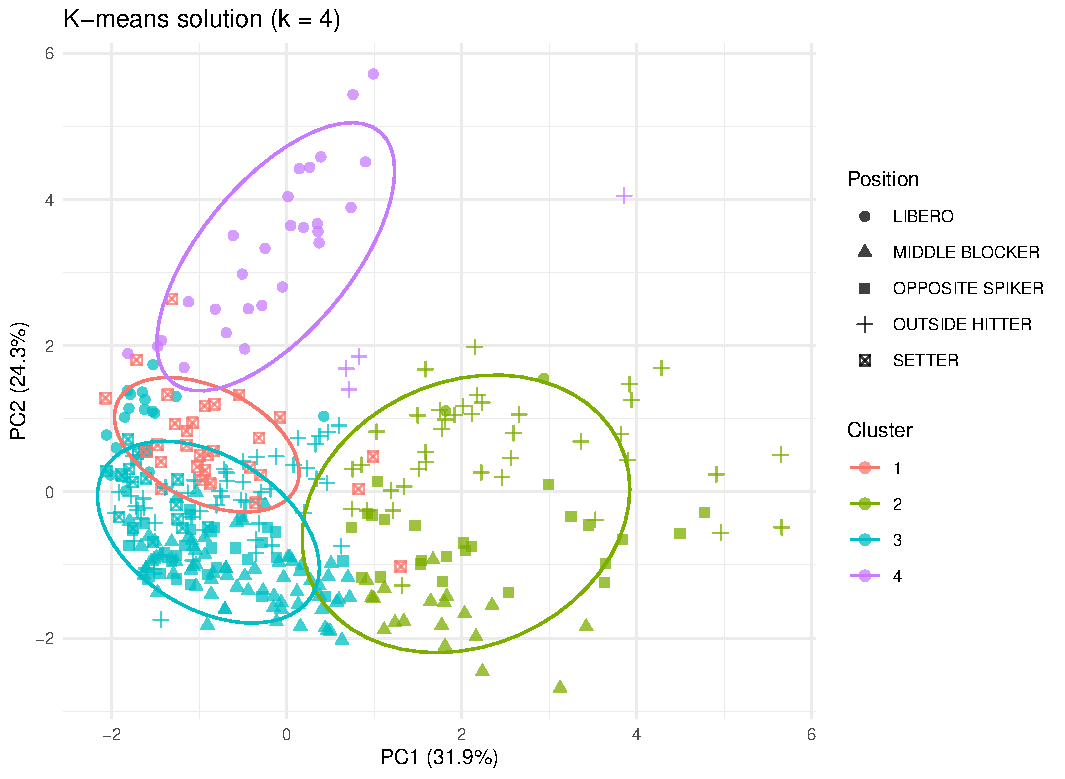
\includegraphics[width=.72\textwidth]{../../outputs/exercise3/kmeans_pca.pdf}
\caption{PCA display of the four-cluster K-means solution; position is shown only for post-hoc interpretation.}\label{fig:km}\end{figure}

\section{Comparison with DBSCAN}
DBSCAN used the same standardised variables. Following the dimensionality rule $\mathrm{minPts}=2p$, $\mathrm{minPts}=16$; an elbow in the sorted 15-nearest-neighbour distances gave $\epsilon=2.664$. DBSCAN produced one connected dense cluster containing 333 players and six noise players (1.77\% of the sample) (Figure~\ref{fig:db}). Its adjusted Rand index against K-means is only .028, demonstrating almost no partition agreement. This is not a failure of either algorithm: K-means is forced to partition all observations into compact Voronoi groups, whereas DBSCAN asks whether density-separated regions exist. Here, player profiles form connected gradients with a few sparse extremes rather than four density islands.
\begin{figure}[!htbp]\centering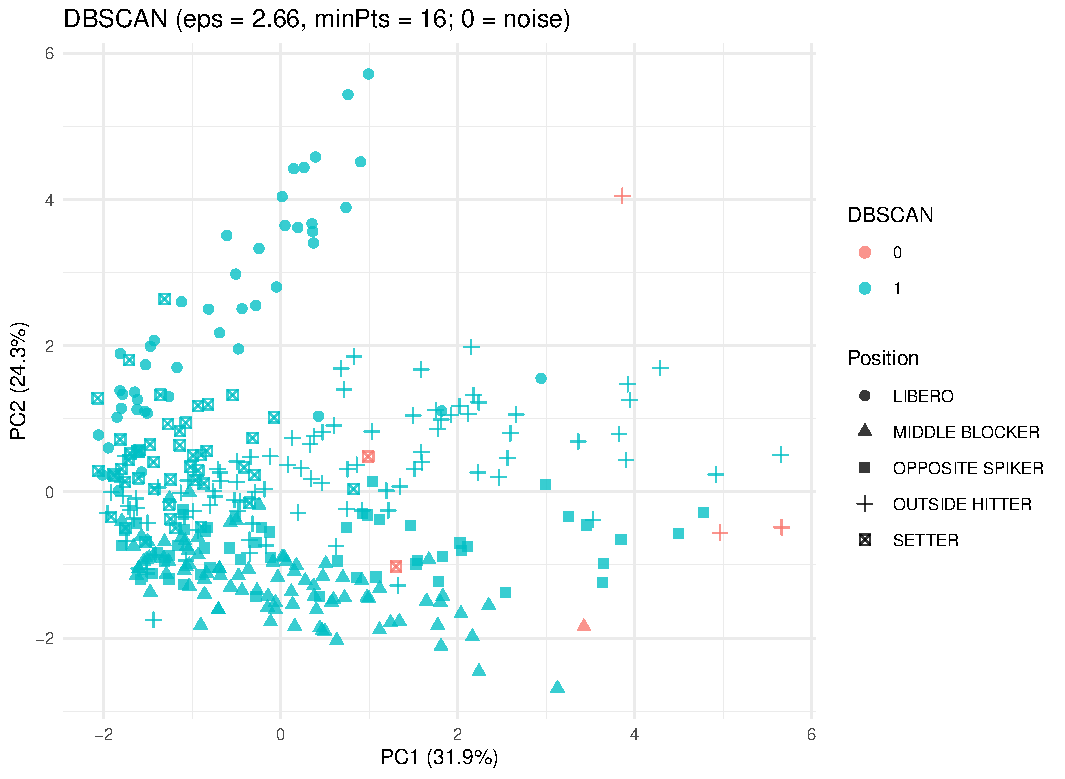
\includegraphics[width=.72\textwidth]{../../outputs/exercise3/dbscan_pca.pdf}
\caption{DBSCAN projected onto the same PCA plane; label 0 denotes noise.}\label{fig:db}\end{figure}

\section{Alignment with position and country}
The post-hoc position comparison (Figure~\ref{fig:align}) strongly supports the functional interpretation: Cram\'er's $V=.607$. Cluster 1 consists entirely of setters; 87.1\% of Cluster 4 are liberos; Cluster 2 concentrates hitters and blockers. This is external face validity, not supervised accuracy. Country alignment is weak ($V=.134$), compared with the much stronger position alignment ($V=.607$): each national team contains several roles and therefore contributes to several clusters. Country differences can also reflect roster composition and playing opportunity, so a country's cluster proportions should not be interpreted as national quality.
\begin{figure}[!htbp]\centering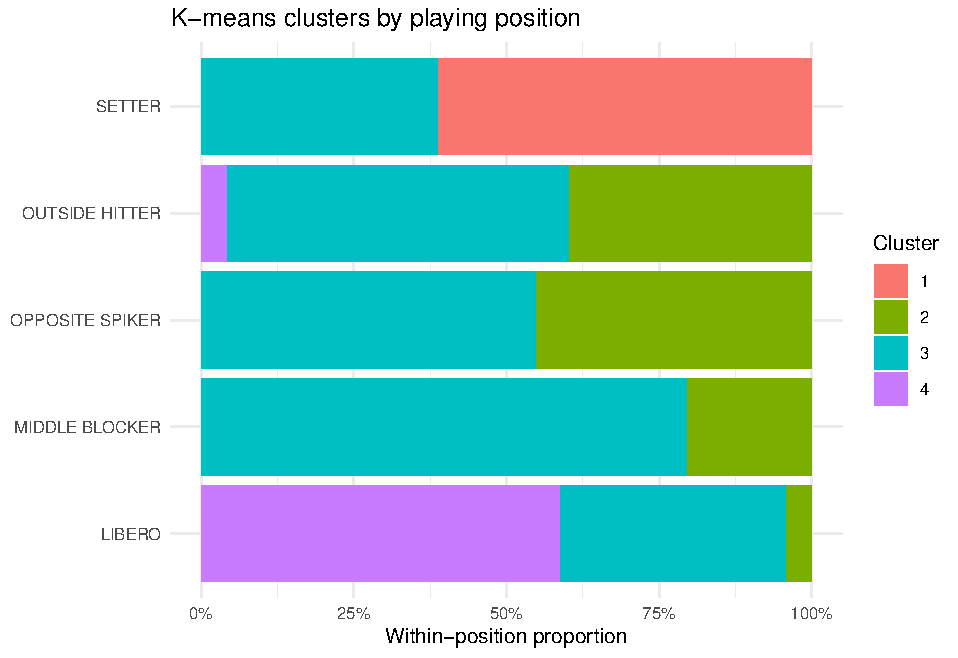
\includegraphics[width=.65\textwidth]{../../outputs/exercise3/clusters_by_position.pdf}
\caption{Within-position K-means composition.}\label{fig:align}\end{figure}

\FloatBarrier
\section{Conclusion}
Four K-means clusters provide the clearest tested compact partition and recover recognisable volleyball role profiles. DBSCAN instead finds a single connected population plus six unusual profiles. Together, the methods suggest meaningful role gradients but limited evidence for sharply density-separated athlete types.
\section*{Statement of Contributions}
Indudhara Swamy Vivekananda conducted preprocessing, clustering, validation, visualisation, interpretation, and report preparation. This statement must be updated if additional group members contributed.
\end{document}

